% Dissertation LaTeX Template
% Author: Karol Cieslik
% LinkedIn: https://www.linkedin.com/in/karolcieslik/
% I have developed this template over the years.
% I hope that it will be useful for others. 
% It works both for thesis in English and in Polish.

\documentclass[11pt,twoside]{report}
% \usepackage[landscape]{geometry}
\usepackage[left=35mm,top=25mm,right=25mm,bottom=25mm]{geometry}
\usepackage{indentfirst}
\usepackage{polski}
\usepackage[polish,english]{babel}
\usepackage{amsmath} % Required for some math elements 
\usepackage[titletoc]{appendix}
\usepackage{rotating} 
\usepackage[
protrusion=true,
activate={true,nocompatibility},
final,
tracking=true,
kerning=true,
spacing=true,
factor=1100]{microtype}
\SetTracking{encoding={*}, shape=sc}{40}
\newsavebox{\myhbar}
\savebox{\myhbar}{$\hbar$}
\renewcommand*{\hbar}{\mathalpha{\usebox{\myhbar}}}
\usepackage[utf8]{inputenc}
\usepackage[version=3]{mhchem} % Package for chemical equation typesetting
\usepackage{siunitx} % Provides the \SI{}{} and \si{} command for typesetting SI units
\usepackage{graphicx} % Required for the inclusion of images
\usepackage{float}
\usepackage{wrapfig}
\usepackage{fancyhdr} % Custom headers and footers
\pagestyle{fancyplain} % Makes all pages in the document conform to the custom headers and footers
\setlength\parindent{0.75cm}
\linespread{1.15}
\fancyhf{} 
\fancyfoot[R]{\thepage}
\pagestyle{fancy}
\fancyhead[L]{\scshape\nouppercase{\rightmark}}
\setlength{\headheight}{13pt} 
\usepackage{titlesec}
 \titleformat{\chapter}[display]   
{\normalfont\huge\bfseries}{\chaptertitlename\ \thechapter}{20pt}{\Huge}   
\titlespacing*{\chapter}{0pt}{-20pt}{20pt}
\usepackage{caption}
\usepackage[font={small}]{caption}
\usepackage{enumerate}
\usepackage{multirow}
 \graphicspath{{wykresy/}}
   \usepackage[unicode=true]{hyperref}
\renewcommand\refname{Bibliografia}
\newcommand{\horrule}[1]{\rule{\linewidth}{#1}} 

% In the SI package you can declare your own units which comes in handy
\DeclareSIUnit{\ions}{ions} 
\DeclareSIUnit{\langmuir}{L} 



\usepackage{hypcap}
\usepackage{booktabs}
\newcommand\doubleRule{\toprule\toprule}
\newcommand\doublerule{\toprule\specialrule{\heavyrulewidth}{\doublerulesep}{0.4em}}
\newcommand{\ra}[1]{\renewcommand{\arraystretch}{#1}}
\AtBeginDocument{\addtocontents{toc}{\protect\thispagestyle{empty}}}
\usepackage{emptypage}
\usepackage{etoolbox}
\patchcmd{\chapter}{plain}{plain}{}{}
\usepackage{hyperref}
\setlength{\belowcaptionskip}{-10pt}
\usepackage{enumitem}
\setlist[itemize]{noitemsep, topsep=0pt}
\usepackage{booktabs,caption}
\usepackage[flushleft]{threeparttable}
\usepackage{acronym} 

%this package is just useful for the template 

\usepackage{lipsum}  

\begin{document}
	\begin{titlepage}
	\centering
	%\vspace*{1cm}
	\Large
	\textsc{Northumbria University \\ Department of Engineering and Environment} \\ \vspace*{1\baselineskip}
	
	
\includegraphics[width=0.25\textwidth,height=0.25\textheight,keepaspectratio]{uj_logo.png}
	
	\horrule{0.5pt} \\[0.4cm] % Thin top horizontal rule
	\Huge  Sensing Metasurfaces: Architectures for Thermo-photovoltaic Modules with Environmental Sensing (Working Title) \\ % Doctoral thesis
	\horrule{2pt} \\[0.5cm] % Thick bottom horizontal rule
	
	\Large{Project Proposal \\ \textit{submitted by}}  % Doctoral thesis
	\vspace*{1\baselineskip}
	
	\LARGE \textbf{Nick L. Theodorou} \\
		\vspace*{1\baselineskip}

	\Large{\textit{supervised by:} \\ Prof. Hamdi Torun \\}
		
	\vspace*{2\baselineskip}
	\Large{Newcastle, 2024}
	
    \end{titlepage}

    
% \shipout\null

% \newpage
% \thispagestyle{empty}
% \vspace*{30px}
% \begin{flushleft}
% \large{Department Name\\
% University name}
% \end{flushleft}
% \vspace*{1\baselineskip}


% \hspace{5.31cm}{\textbf{\Large{Declaration}}

% \vspace*{15px}

% {\large{\lipsum[5]

% \lipsum[12]

% \vspace*{25px}
% \begin{center}
% 	\begin{tabular}{lr}
% 		................................~~~~~~~~~~~~~~~~~~~~~~~~~~~~~~~~~~~~~~&
% 		.......................................... \\
% 		{~~~~~~~~City, date} & {Your signature~~~~~~~}
% 	\end{tabular}
% \end{center}
% \noindent \hfill 


% \noindent  \hfill }}}
% \\

%the numbering should be different in the sections before the main body of the dissertation


\pagenumbering{roman}
\setcounter{page}{0}

% \clearpage
% \phantomsection
% \addcontentsline{toc}{chapter}{Acknowledgements}
% \chapter*{Acknowledgements}

\lipsum[1-3]  
% \clearpage
% \phantomsection
% \addcontentsline{toc}{chapter}{Acknowledgements in another language}
% \include{chapters/Acknowledgements2}  
\clearpage
\phantomsection
\addcontentsline{toc}{chapter}{Statement of Distinctiveness}
\chapter*{Statement of Distinctiveness} 
 The project aims to address climate change by focusing on the development of metasurfaces for renewable energy applications, highlighting their potential for waste heat recovery. Prior art is discussed; the document covers the history and development of metamaterials, metasurfaces, and the emerging prospect of their application in environmental sensing and energy harvesting. The project aspires to address environmental challenges through an innovative framework of metasurface design.








  
% \clearpage
% \phantomsection
% \addcontentsline{toc}{chapter}{Abstract in another language}
% \include{chapters/Abstract2}   
\clearpage
\phantomsection
\addcontentsline{toc}{chapter}{Acronyms}
\chapter*{Acronyms}
\begin{acronym}
% \acro{GHG} {Green House Gas}
% \acro{MM} {Meta Material}
% \acro{SAW} {Surface Acoustic Wave}
\acro{MM}{Meta Material}
\acro{SAW}{Surface Acoustic Wave}
\acro{SHG}{Second Harmonic Generation}
\acro{TPV}{Thermo Photo Voltaic}
\end{acronym}          

%the style of numbering of pages

\pagenumbering{arabic}

%you can add some chapters 

\tableofcontents

%you can add some chapters 

 \pagenumbering{arabic}
\chapter{Project Proposal}

\section{What’s the potential for this project?}

Climate change is already beginning to affect global systems beyond the observed average annual temperature rises \cite{ipcc2021},\cite{nrdc2023effects}.
    Net Zero means taking necessary actions to install systems which are designed to ensure “any emissions would be balanced by schemes to offset an equivalent amount of green house gases (GHG) from the atmosphere”
\cite{ukgov2023}.

This complex problem has multiple facets, however one approach is to triage the source of GHG contributions, for example:
\\
To produce 1000 tons of steel, up to 1850 tons of CO2 is produced \cite{mckinsey2020decarbonization}. 
In 2019, 1.875 Billion tons of steel was produced. This means that at least 3.375 billion tons of CO2 was produced. 37 Billion metric tons represents the global GHG emissions in both 2019 \& 2022 (2020: 35 Billion) \cite{hausfather2022global}. 65\% of emissions is attributable to CO2 and fossil fuel \cite{Jones2023CO2}.
\\
\\
Waste heat recovery systems represent a significant environmental opportunity, and one that is economically aligned with industry. Waste heat reclamation would reduce operational costs and energy consumption in steel manufacture alone by 45\% \cite{doe2008wasteheat}. 
\\
This project plan outlines a path for systematic search and demonstration of value-accretive metasurfaces suitable for such renewable energy settings, namely photovoltaics.

To date, all but one commercial thermo-photovoltaic (TPV) system has been built (by JX Crystals) - based on an emitter material composite designed to be ``well-matched'' for Gallium Antimonide (GaSb) cells \cite{ferguson_matched_1997}, \cite{fraas2002thermophotovoltaics}. However, Antora energy is soon expected to begin production after a 40\% efficient TPV system was demonstrated - an important threshold for being comparable to steam-driven turbines \cite{thermophotovoltaic2022efficiency}, \cite{pv_magazine_2023_thermophotovoltaic}. With no moving parts, and high theoretical efficiency ceiling, TPV is a promising candidate for the next wave of engineering effort to carefully consider, with still considerable headroom for improvement.
\\
On the other hand, the installed base of solar photovoltaics already (as of 2022) exceeds 1.185 Terrawatts, accounting for 6\% of global needs (up from 3\% in 2019) \cite{ieapvps2023}, \cite{ieapvps2020}. This technology is not without downsides; ways to improve efficiency and reduce environmental cost must be found.

Research impact for this project will follow from answers to the intriguing questions posed. What unique sensing, detection, and energy harvesting capabilities exist? Is `dynamic' tunability required? Can the design of metasurfaces be systematically customised to achieve desired absorption responses at specific frequency ranges? The unifying theme: is it viable to design manufacturable metasurface architectures that enhance photovoltaic systems?


\section{Background}

Theoretical ‘Metamaterials’ were suggested in the 1960s, but it was unknown how practical realisation could be accomplished \cite{veselago1968}. By the mid-1990s it was realised geometric features, rather than chemical composition alone, could be utilised to architect the response of incident waves (Guo2023 \cite{Guo2023}). Collaboration between Imperial College London and the Marconi Company revealed that, within the realm stealth technology, the geometric contribution of thin carbon fibres significantly influenced the structure's electromagnetic response; more so than the underlying characteristic properties of the material itself. Meta simply means to `go beyond’ naturally-occurring materials.

Experimental exhibition of a metamaterial with induced negative index of refraction was achieved shortly after; simultaneously negative electric and magnetic responses within a composite of non-magnetic materials (Smith2000 \cite{smith2000}, \cite{shelby2001}).
Metasurfaces (two-dimensional equivalents), have recently been used to demonstrate seismic cloaking (earthquake prevention) by controlling surface waves on the earth \cite{palermo2018}.
Given the complexity of attaining Net Zero there was never a more pertinent time to access the viability of metasurface designs.
In the realm of energy-harvesting, metamaterials have been engineered with perfect absorptance; transmission and reflection may be suppressed entirely. At the same time, they possess excellent characteristics that can break the thickness limitation of traditional bulky absorption devices. A comprehensive and up-to-date overview of meta-absorber achievements may be readily found (Wang2023) \cite{wang2023broadband}.

\begin{figure} [!h]
	\centering
	%\captionsetup{justification=centering}
	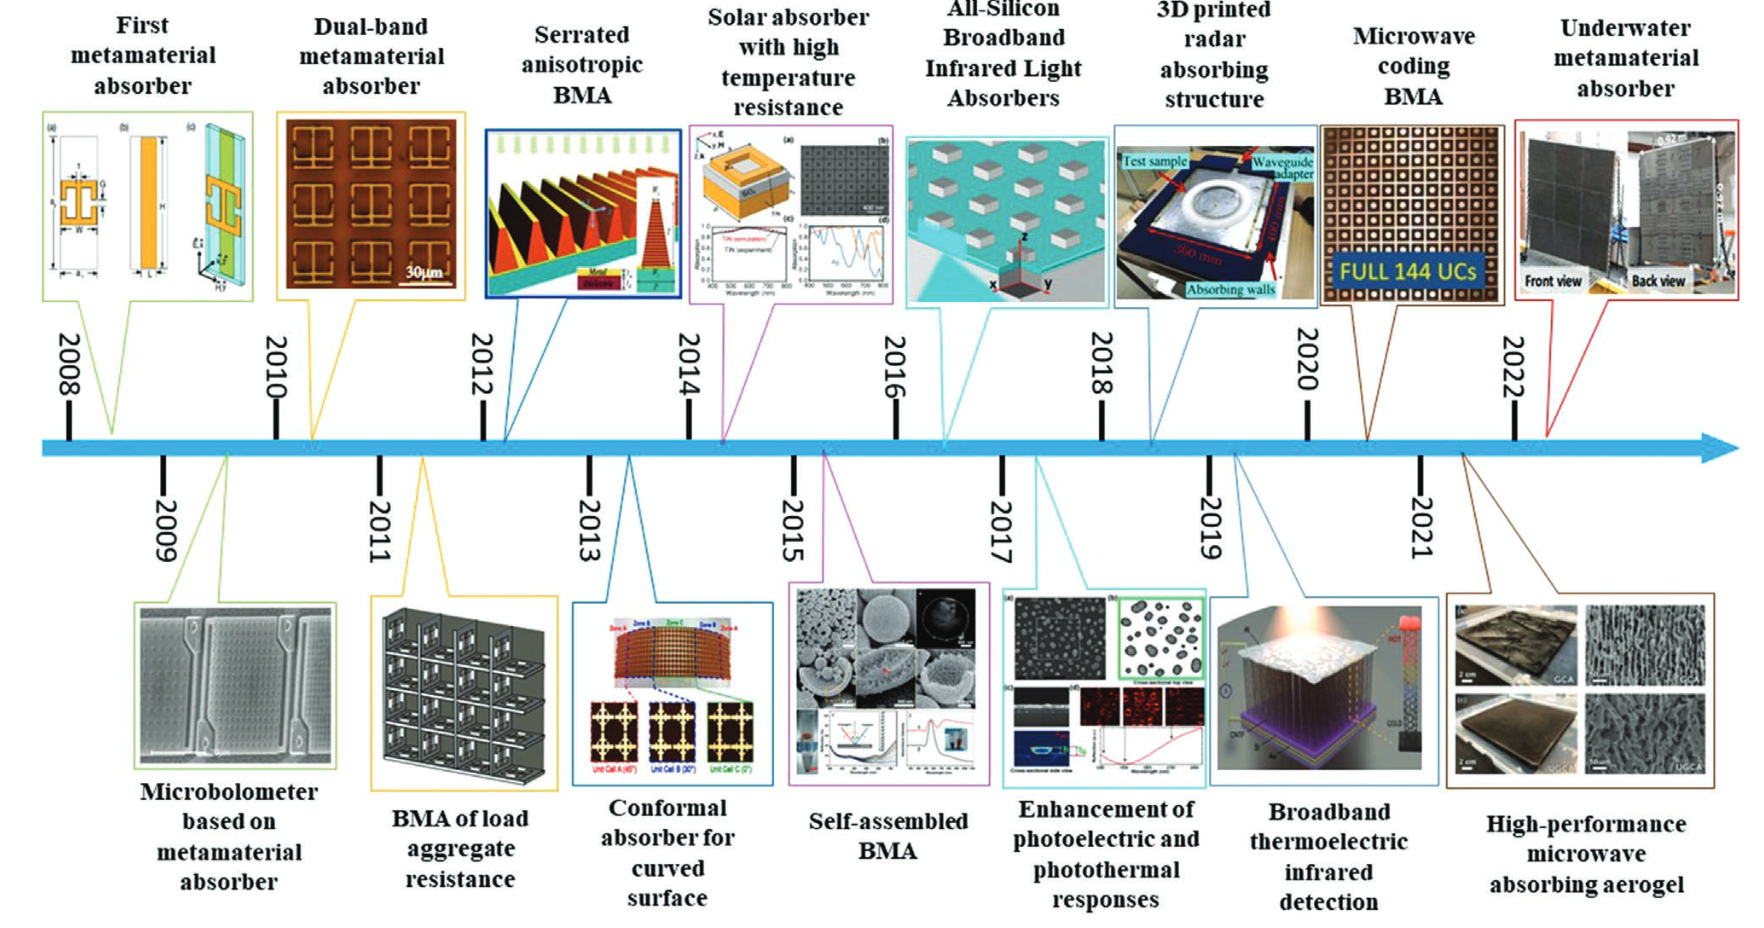
\includegraphics[width=14cm,height=8cm,keepaspectratio]{figures/introduction/achievements}
	\setlength\belowcaptionskip{3pt}
	\caption{Achievements to date in metamaterial absorbers \cite{wang2023broadband}}
	\label{some-figure}
\end{figure}

This resource highlights the necessity for a deeper exploration. This project will focus on the design, functionality, and application of these materials. Wang2023 underscores the importance of developing multifunctional absorption devices, capable of integrating various applications such as energy harvesting, photodetectors, stealth technology. This project will focus on opportunities for tunable and reconfigurable metamaterials that adapt to environmental changes - thereby enhancing the performance and scope of these absorbers.

\begin{figure} [!h]
	\centering
	%\captionsetup{justification=centering}
	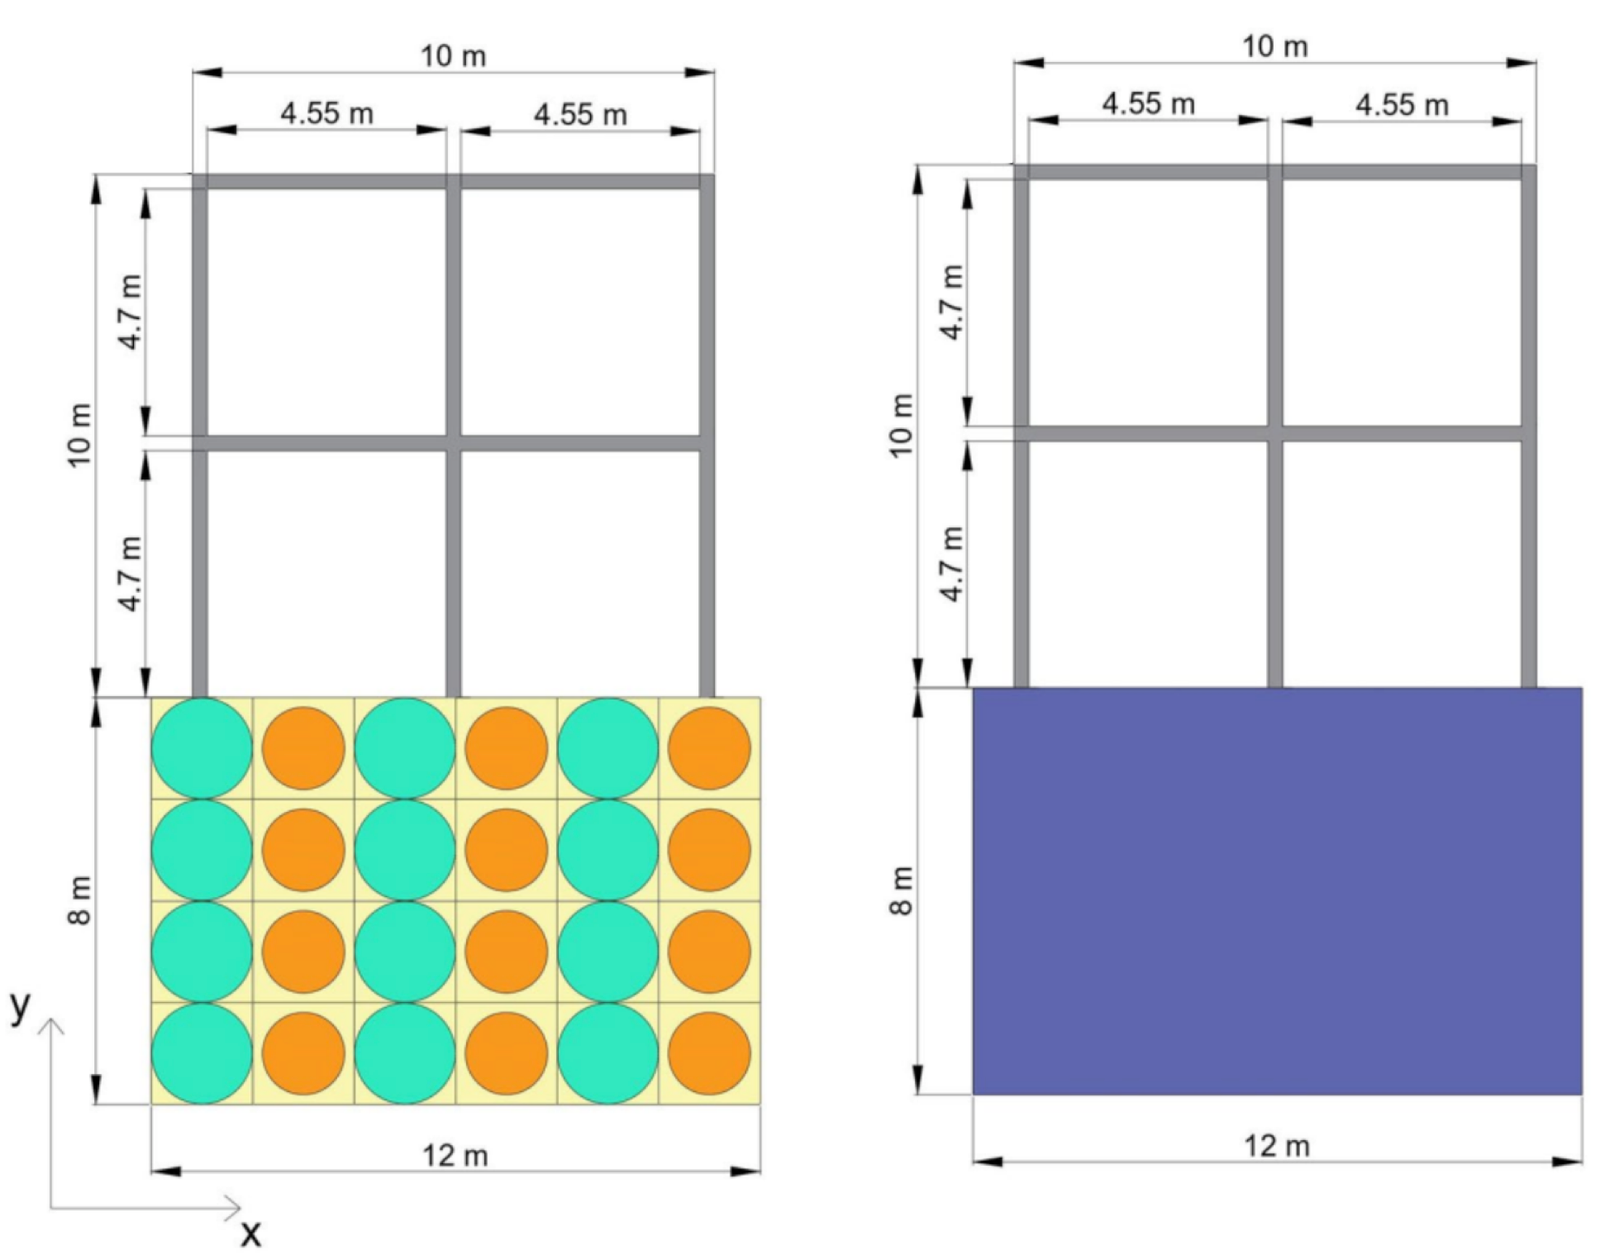
\includegraphics[width=14cm,height=8cm,keepaspectratio]{figures/introduction/cloak.png}
	\setlength\belowcaptionskip{3pt}
	\caption{Illustrating the potential of metamaterials: Steel frame on metamaterial foundation (a),  concrete foundation (b). (Gupta2023 \cite{Gupta2023}). }
	\label{some-figure}
\end{figure}









% Here the Equation \ref{reaction-oxidation-sto} starts:
% \begin{equation}
% 	k \cdot \ce{ SrTiO3} \ce{->} p \cdot \ce{ SrTiO3}  +   q \cdot \ce{SrO (SrTiO3)_n} +  q \cdot \ce{TiO2},
% 	\label{reaction-oxidation-sto}
% \end{equation}
% where $k = q\cdot (n+1) + p$. And here it ends.
%  We are in the Section \ref{section-with-figure} with Figure \ref{some-figure}.



\section{Aims and Objectives} \label{section-with-figure}

Metamaterials are unique for the fact their tailored electromagnetic response can be scaled across the electromagnetic spectrum. Resonant structures may be varied by way of material choices, unit cell geometry and size. Unit cell sizes vary inversely with the resulting resonant frequency value. 
For TPV cells based on Gallium antimonide (GaSb) this would be around 176.5 THz or 1.7 $\mu$m; a unit cell period would need to be smaller than this length. Selected fabrication methods should be commensurate with the resolution requirements of geometric features within a unit cell. 

The focus of the project is to construct a framework of metasurface design; to find absorbers that closely match target photovoltaic cells. Robustness of match will be investigated in the presence of environmental changes to the system; when changes are detected, designs serve as sensors. Tunability mechanisms for measuring or mitigating the effect of environment changes on electromagnetic response will be considered. These include fermi level \cite{Nie2024}, doping concentrations \cite{MoS2}, mechanical strain \cite{Amir2023}, and others.

For experimental validation, in Year 1 (2024) fabrication methods to be ultilised are already available. UV photolithography is anticipated to serve for devices with a resolution requirement of 5-10$\mu$m, while Atomic Layer Deposition will conformally coat an entire structure with material in 1nm steps. 

In following years alternate techniques e.g. Focused Ion Beam (FIB) are anticipated to become available to attain sub-1.7 $\mu$m geometric features. Given this initial constraint, the primary objective is to fabricate devices that are scaled up by x20 times. Through simulation work, equivalence between scaled up and scaled down designs shall be demonstrated. 

To accelerate a proficiency in running a sensing experiment, work will begin on readily available Surface Acoustic Wave (SAW) devices (millimetres to centimetres in size). The influence of water, fog, and ice will be studied for how they alter absorptivity. It is essential to consider how environment factors will play a role in real-world thermophotovoltaic applications - as coupled modes would be confounded by environmental factors, most likely. When resonator devices `couple' there are emergent resonant modes. Coupling by Surface Acoustic Waves not only modulates resonator eigenfrequencies (dispersive coupling) but also their damping (dissipative coupling) \cite{Rieger2022SurfaceAW}. `Optimised' metasurface designs would yield specific absorptivity and emissivity characteristics, for efficient energy harvesting (or sensing) at these frequencies. 

Deep Learning methods for the objective of parameter search through inverse design is emerging as a viable alternative to traditional Particle-In-Cell-Simulations \cite{Nadell2019}. In the context of thermophotovoltaic systems this would relate to designing refractory metamaterials capable of surviving high radiator temperatures while attaining suitable emitter frequencies, to match photovoltaic bandgaps (Coutts1999 \cite{coutts1999}).

\begin{figure} [!h]
	\centering
	%\captionsetup{justification=centering}
	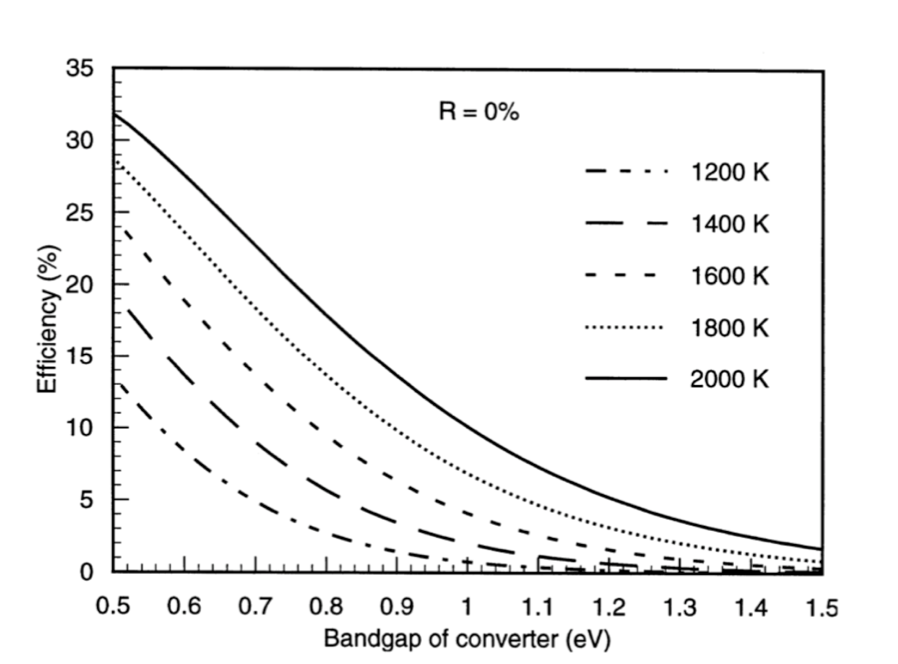
\includegraphics[width=14cm,height=8cm,keepaspectratio]{figures/introduction/tpv1.png}
	\setlength\belowcaptionskip{3pt}
	\caption{Modelled variation of efficiency with bandgap of the converter. The radiator temperature is treated parametrically. No sub-bandgap photons are returned to the radiator (Coutts1999 \cite{coutts1999})}
	\label{some-figure}
\end{figure}

By Year 2.5 (July 2025) nano-scale demonstrations will begin, with an emphasis on performant designs for mission-critical aspects of the thermophotovoltaic system; photon recycling, higher radiator temperatures, and targeted bandgap-matching. There shall be a consideration for necessary and achievable sensing or detection capabilities within the context of envisioned operational settings for TPV systems. The focus will be to identify sensing capabilities that are can be readily integrated via absorption tuning. For example, carbon auditing. 

One envisioned setting for thermophotovoltaics is industrial steel manufacture. Carbon auditing would relate to the varying rate of waste heat recycling. It may prove useful to account recycled heat for carbon auditing purposes. It is worth noting steel comes in various quality grades, due to energy savings higher quality steel could become more affordable, and higher uptake in quality steel can result in a lower need for steel use overall; consequently a smaller environmental footprint.

%Cite: Sir Harry Bhadeshia, Life scientific interview

In Year 3 (2026) attention shall be paid to commercial fabrication techniques. One ‘roll-to-roll’ polymer-based metasurface has been identified \cite{Ma2023}. The author reinforces the potential for ‘trench-like’ structures to be redesigned with active thermal management - a statement that echoes the research gap addressed in this proposal.

The primary question for scaled-up production is whether to recommend “Industry 4.0” or traditional manufacturing. Foundries vary widely in production volumes \cite{wiki:memsfoundries}; high volumes may infer low cost per unit albeit at high overhead. Alternatively, additive manufacturing unlocks ‘mass customisation’. This consideration may become crucial for market adoption at flexible production volumes.

\section*{Design and `Scaled Up' Fabrication (Year 1 and 2):}
\begin{itemize}
	\item Aim: Create a dataset of proposed metasurface designs 
    \item Objective 1: Using forward design, create simulations well matched to external quantum efficiency measurements for a variety of PV cells beginning with GaAs.
    \begin{itemize}
        \item Quantify the match between target and attained absorptivity response curves in terms of mean square error.
    \end{itemize}
    \item Objective 2: Fabricate three proposed designs in year 1 (2024) using photolithography and other readily available techniques.
    \begin{itemize}
        \item Use results from completed SAW device experiments to propose suitable sensing experiments for these devices.
    \end{itemize} 
    \item Objective 3: Through simulation, demonstrate correspondence between scaled up and scaled down versions of unit cell geometries. Seek to represent the mathematical relationship between geometrical features and resonant frequencies (wideband or narrowband), thereby demonstrating tunability.
\end{itemize}
\section*{`Scaled down' Fabrication and Characterisation (Year 2.5 and Year 3:}
\begin{itemize}
	\item Aim: Expand the framework - design, fabrication, characterisation.
    \item Objective 4: By end of year 3 (2026) fabricate three nano-structured metasurface designs using FIB or Electron Beam Lithography (EBL).
    \item Objective 5: Measure and characterise thermalisation loss / and suppression of the metasurface-PV system compared to the standalone PV cell.
\end{itemize}
\section{Indicative Methodology}


\subsection{Literature Review}
\begin{itemize}
    \item Review literature on Metasurface design and application of metasurfaces in thermophotovoltaic systems.
    \item Analyse relevant Machine Learning methods for parameter search in Metasurface design.
    \item Investigate the current state and future prospects of sensing using metamaterials, particularly in the context of thermophotovoltaic systems.
    \item Review fabrication techniques suitable for metasurface construction, with an emphasis on achieving the necessary geometric feature sizes.
    \item Examine methods for tunability in metasurfaces, such as doping concentrations, bias voltage, and their implications for environmental sensing.
\end{itemize}

\subsection{Simulation and Modeling}
\begin{itemize}
    \item Utilise simulation software to model and simulate proposed designs.
    \item Where possible validate simulations using data from real experiments or values obtained from published literature.
    \item Refine the models based on feedback from fabrication and characterisation efforts.
    \item Explore the scalability of unit cell designs through simulation, demonstrating the equivalence between scaled-up and scaled-down models and their resonant frequencies.
    \item Establish a comprehensive understanding of solver operations in simulation software and physical models.
\end{itemize}


\subsection{Experimental Validation}
\begin{itemize}
    \item In Year 1, utilize available UV photolithography and Atomic Layer Deposition techniques for initial metasurface fabrication, targeting larger unit cell structures suitable for scaled-up designs.
    \item Begin preliminary environmental sensing experiments using available Surface Acoustic Wave devices, focusing on the impact of environmental changes on absorptivity.
    \item By Year 2.5, transition to fabrication techniques capable of sub-micron resolution, like Focused Ion Beam, to create nano-structured metasurfaces for TPV applications.
\end{itemize}

\subsection{Environmental Sensing Development}
\begin{itemize}
    \item Develop sensing algorithms to detect and quantify environmental changes, leveraging the tunable properties of metasurfaces.
    \item Integrate these sensing capabilities into the metasurface design to facilitate environmental monitoring.
\end{itemize}

\subsection{Collaboration \& Characterisation}
\begin{itemize}
    \item Collaborate with expert researchers to gain access and training to any specialist equipment that is required.
\end{itemize}

\subsection{Application of Metasurface Framework}
\begin{itemize}
    \item Apply the developed framework to recommend and fabricate structures with specific functionalities, namely enhanced TPV efficiency.
    \item Consider the suitability of these designs within industrial settings, such as steel manufacturing.
\end{itemize}

\subsection{Lab-Scale to Commercial Fabrication Consideration}
\begin{itemize}
    \item In Year 3 (2026), evaluate the feasibility of transitioning from lab-scale fabrication to commercial production, considering techniques such as roll-to-roll manufacturing for polymer-based metasurfaces.
    \item Evaluate the potential for industrial upscaling, focusing on cost and adaptability to different production volumes and market needs.
\end{itemize}



\section{Research Plan}


\begin{figure}[h]
    \centering
    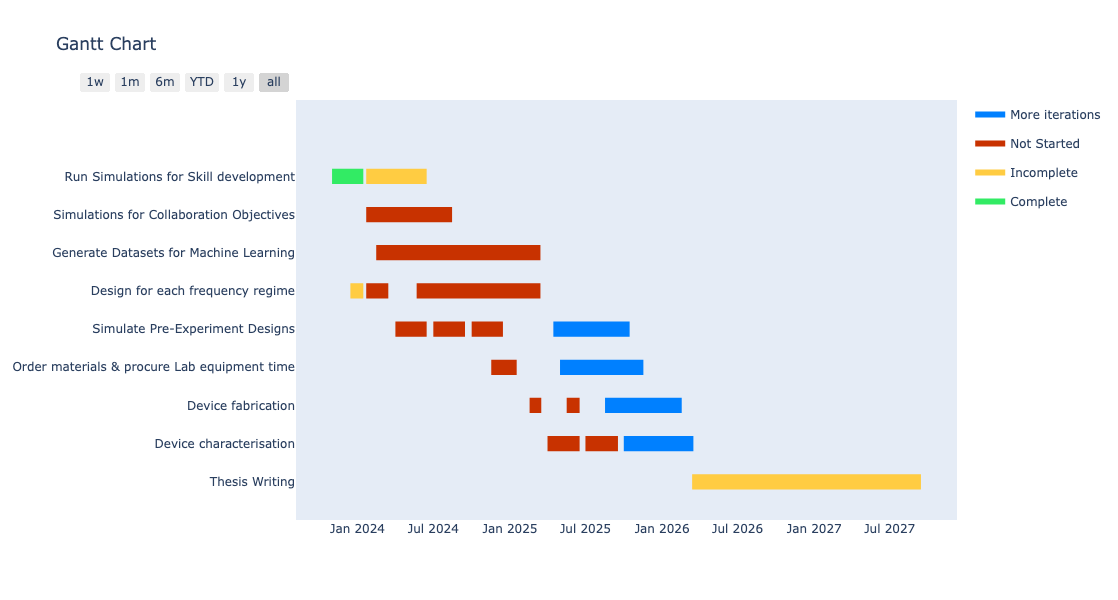
\includegraphics[width=\textwidth]{figures/introduction/gantt.png}
    \caption{Gantt Chart}
    \label{fig:your_label}
\end{figure}


\begin{sidewaysfigure}
    \centering
    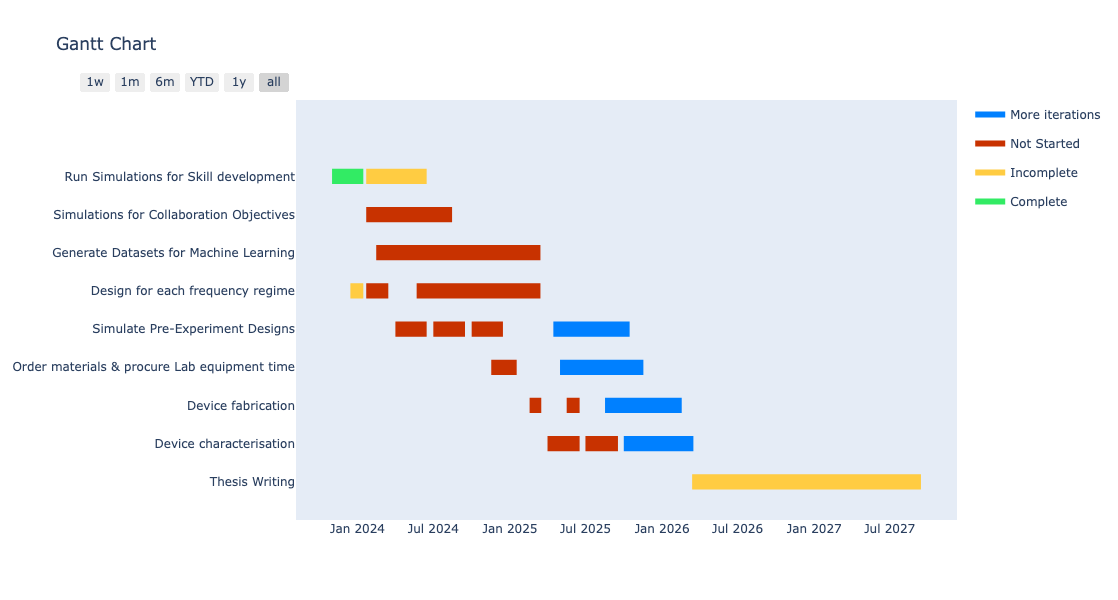
\includegraphics[width=\textwidth]{figures/introduction/gantt.png}
    \caption{Gantt Chart}
    \label{fig:your_label}
\end{sidewaysfigure}

% \chapter{Experimental}

\lipsum[7]

\section{Something about the experiment }

\lipsum[8]
 
\subsection{A subsection with a table } 

\lipsum[9-10]


\vspace{7pt}
\begin{table}[!h]
	\centering
	\ra{1.1}
	\caption{The comparison of published desorption energy and pre-exponential factor of 6P multilayer with the ones obtained from manual linear heating and passive cooling of the 6P powder. The values of kinetic parameters calculated using heating curves obtained based on different assumptions.}
	\label{arr_tab_6p}
	\vspace{-5pt}
	\resizebox{\textwidth}{!}{%
		\begin{tabular}{@{}lS[table-format=1.3]S@{}}
			\doublerule
			& {Desorption energy (\si{\electronvolt})}   & {Pre-exponential factor (\si{\per \second})}    \\
			\midrule
			Manual linear heating       & 3.54(2) & \SI{6.2(5)E33}{}   \\
			Manual linear heating  (different assumptions)      &  &    \\
			\hspace{1cm}Linear region after \SI{2}{min}, offset \SI{30}{\celsius}       & 3.93(2) & \SI{2.8(2)E35}{} \\
			\hspace{1cm}Linear region after \SI{2}{min}, offset \SI{-30}{\celsius}        & 3.18(2) &  \SI{1.4(1)E32}{} \\
			\hspace{1cm}Linear region after \SI{3}{min}, offset \SI{0}{\celsius}     & 2.84(2) & \SI{2.8(2)E27}{} \\		
			\hspace{1cm}Linear region after \SI{1}{min}, offset \SI{0}{\celsius}   & 4.10(2) & \SI{6.4(5)E38}{} \\
			Manual linear heating  (with estimated error)      & 3.5(7)  & \phantom{(0.00..)}{$6 \times 10^{33(5)}$}  \\ \midrule
			Passive cooling       & 3.17(2) & \SI{2.4\pm0.2E32}{} \\
			Passive cooling   (with estimated error)      & 3.2(2)  & \phantom{(0.00..)}{$2 \times 10^{32(1)}$}  \\ \midrule
			6P multilayer, A. Winkler (2015)    & 2.4     & \phantom{(00.)}\SI{6E25}{} \\
			\bottomrule   
	\end{tabular}}
\end{table}



\textbf{The table shows how one can use the SI package to align values in a column to a symbol or a decimal point. }



\subsection{A giant complicated table for a whole page}

\lipsum[61]


\begingroup
\renewcommand*{\arraystretch}{1.4}

\begin{sidewaystable}[]
	\centering
	\ra{1.1}	
	\caption{Summary of the used annealing methods describing their characteristics in the context of oxide reduction experiments.}
	\label{annealing-summary}
	\resizebox{\textwidth}{!}{%
		\begin{tabular}{@{}lllllll@{}}\doublerule
			Annealing method                                                          & Sample                                                            & Max temp. of sample                                                                                                                                                                     & Temp. uniformity                                                                   & Temp. of getter                                                                                                       & Cleanliness                                                                & ELOP usefulness                                                   \\ \midrule
			\begin{tabular}[c]{@{}l@{}}Current through\\ sample \\ \\ \phantom{empty}\end{tabular} & \begin{tabular}[c]{@{}l@{}}Monocrystal\\ \\ \\ \phantom{empty}\end{tabular} & \begin{tabular}[c]{@{}l@{}}Depending on type of crystals\\ and luck, for \ce{TiO2} on\\ Si \textgreater{}\SI{1350}{\degreeCelsius}, for \ce{SrTiO3} on Si \SI{1250}{\degreeCelsius}\\ was achieved\end{tabular}                          & \begin{tabular}[c]{@{}l@{}}Relatively uniform\\ below \SI{1050}{\degreeCelsius}\\ (approx. \SI{30}{\degreeCelsius})\\ \\ \phantom{empty}\end{tabular} & \begin{tabular}[c]{@{}l@{}}Unknown, but higher\\ than the studied\\ sample's*\\ \phantom{empty}\end{tabular}                                   & \begin{tabular}[c]{@{}l@{}}Clean\\ \\ \\ \phantom{empty}\end{tabular}                & \begin{tabular}[c]{@{}l@{}}Useful \\ \\ \\ \phantom{empty}\end{tabular}     \\ \hline
			\begin{tabular}[c]{@{}l@{}}Electron beam\\ holder\\ \\ \phantom{empty}\end{tabular}    & \begin{tabular}[c]{@{}l@{}}Monocrystal\\ \\ \\ \phantom{empty}\end{tabular} & \begin{tabular}[c]{@{}l@{}}Temp. of sample above \textgreater{}\SI{1350}{\degreeCelsius},\\ temperatures of \SI{1668}{\degreeCelsius}  reached\\ (melting temp of Ti), high temp\\ can be reached without difficulty\end{tabular} & \begin{tabular}[c]{@{}l@{}}Relatively uniform\\ below \SI{1050}{\degreeCelsius}\\ (approx. \SI{30}{\degreeCelsius})\\ \\ \phantom{empty}\end{tabular}  & \begin{tabular}[c]{@{}l@{}}Known, in case of\\ silicon. The same as\\ sample, in case of Ti\\ much higher\end{tabular} & \begin{tabular}[c]{@{}l@{}}Clean\\ \\ \\ \phantom{empty}\end{tabular}                & \begin{tabular}[c]{@{}l@{}}Very useful\\ \\ \\ \phantom{empty}\end{tabular} \\ \hline
			\begin{tabular}[c]{@{}l@{}}Quartz tube\\  \phantom{empty}\end{tabular}                  & \begin{tabular}[c]{@{}l@{}}Monocrystal\\ or powder\end{tabular}    & \begin{tabular}[c]{@{}l@{}}\SI{1150}{\degreeCelsius} can be reached, but above\\ \SI{1000}{\degreeCelsius} Si contamination\end{tabular}                                                                                         & \begin{tabular}[c]{@{}l@{}}Uniform\\ \phantom{empty}\end{tabular}                            & \begin{tabular}[c]{@{}l@{}}Known,\\ the same as sample\end{tabular}                                                  & \begin{tabular}[c]{@{}l@{}}\textgreater{}\SI{1000}{\degreeCelsius}\\ signs of Si\end{tabular} & \begin{tabular}[c]{@{}l@{}}Limited\\ usefulness**\end{tabular}      \\ \hline
			\begin{tabular}[c]{@{}l@{}}Crucible\\ \phantom{empty}\end{tabular}                     & \begin{tabular}[c]{@{}l@{}}Monocrystal\\ or powder\end{tabular}    & \begin{tabular}[c]{@{}l@{}}\SI{1450}{\degreeCelsius} was reached \\ \phantom{empty}\end{tabular}                                                                                                                 & \begin{tabular}[c]{@{}l@{}}Uniform\\ \phantom{empty}\end{tabular}                            & \begin{tabular}[c]{@{}l@{}}Known,\\ the same as sample\end{tabular}                                                  & \begin{tabular}[c]{@{}l@{}}Clean at least\\ till \SI{1450}{\degreeCelsius}***\end{tabular}        & \begin{tabular}[c]{@{}l@{}}Limited\\ usefulness**\end{tabular}     \\ \bottomrule 
		\end{tabular}}
		\begin{tablenotes}
			\small
			\item *The temperature measurement is performed using a pyrometer and the getter crystal is placed under the studied crystal, so its temperature cannot be measured. The getter's temperature is higher than the sample's temperature, as indicated by the color of glowing and the fact that it partially melts even when the temperature of the sample is lower than the getter's melting temperature. 
			\item **The experiments have shown that the getter should have much higher temperature than the perovskite crystal in the study of the growth of nanostructures. When the getter temperature is raised enough for the getter to be active, the temperature of the crystal is so high that the structures are badly defined and contaminated. 
			\item ***The annealing in this method is due to radiation from tungsten wires. It must      be noted that at      high temperatures, tungsten wires begin to sublimate. Contamination with heavy metals was  observed on the surface of monocrystals at high currents passing through wires in another heating system based on the same principle.
		\end{tablenotes}	
\end{sidewaystable}

\endgroup





% \include{chapters/goal}
% \chapter{Results} 

\lipsum[68]

\section{Some section}

\lipsum[69]

\subsection{Its first subsection}

\begin{figure} [!h]
	\centering
	%\captionsetup{justification=centering}
	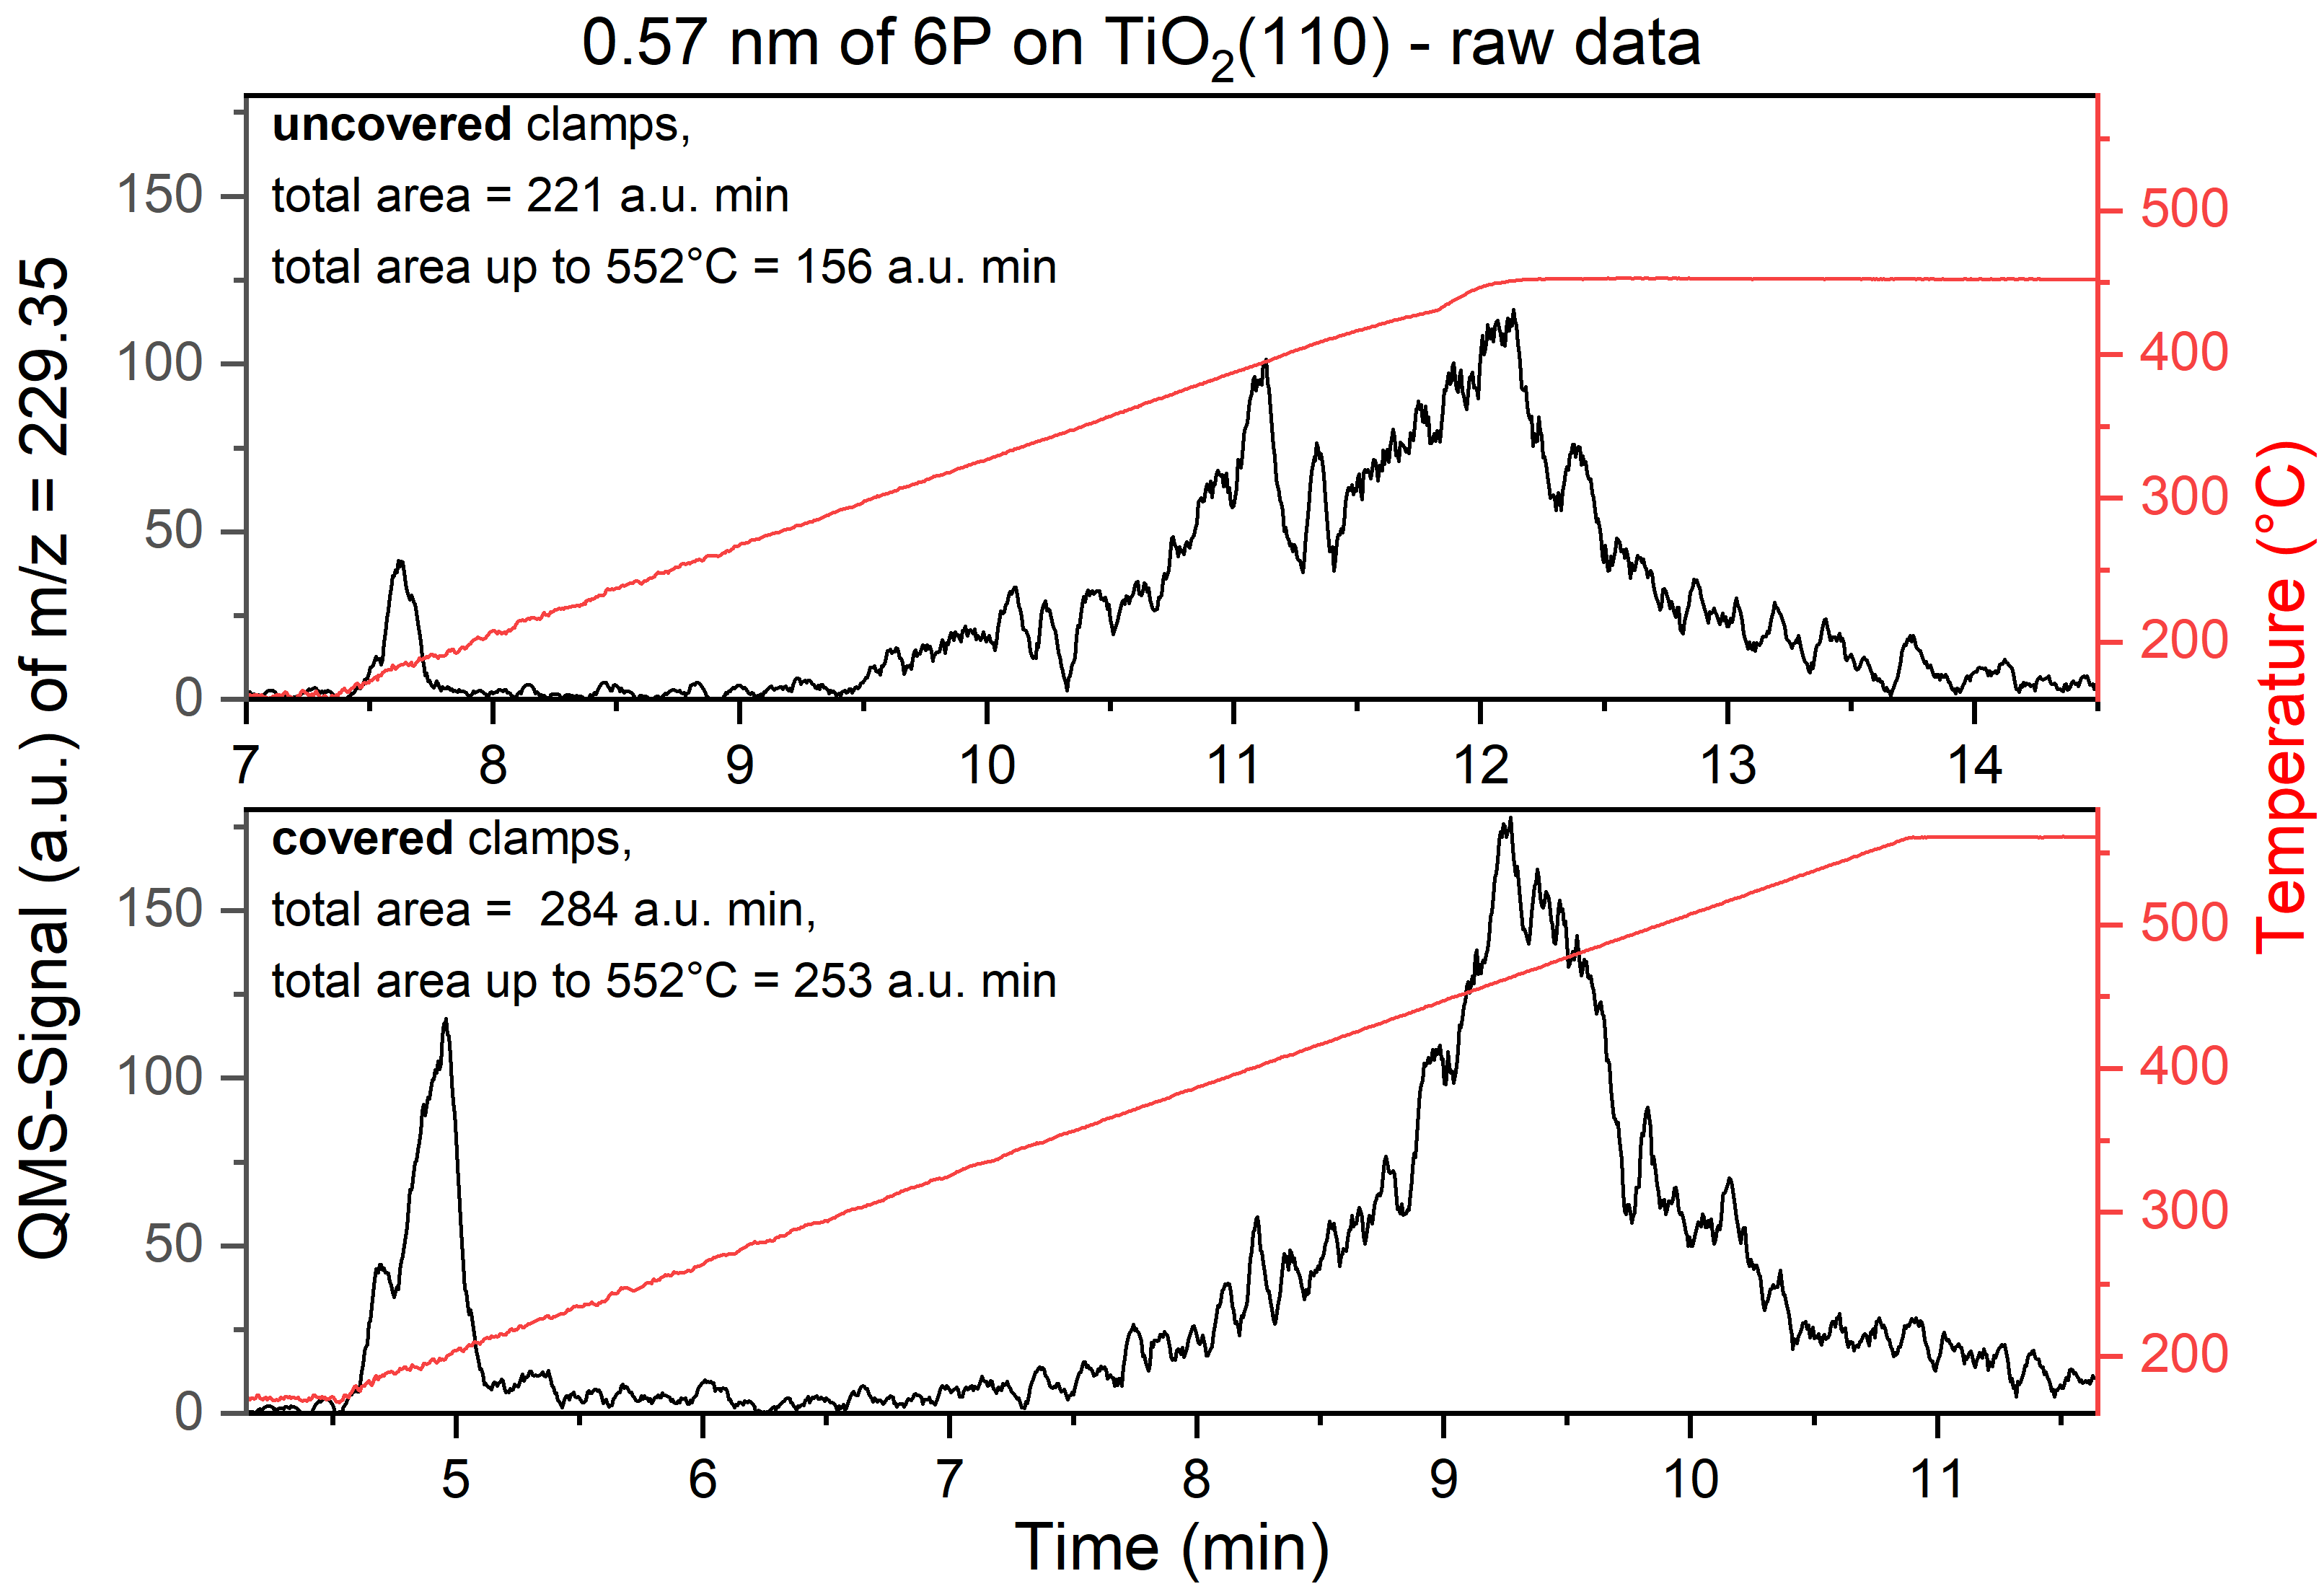
\includegraphics[width=9cm,height=8cm,keepaspectratio]{figures/results/some-graph.png}
	\setlength\belowcaptionskip{3pt}
	\caption{a) the first and b) second part.}
	\label{some-graph}
\end{figure}

Look at the Figure \ref{some-graph}!

\lipsum[70]


\subsection{Its second subsection}
\lipsum[77]



\section{Another section}

\lipsum[78]


% \chapter{Conclusions}


\lipsum[55-59]




\clearpage
\phantomsection
\addcontentsline{toc}{chapter}{Bibliography}


%the bibliography style that you use
\bibliographystyle{ieeetr}

%the file which contains your references

\fancypagestyle{plain}{%
	\renewcommand{\headrulewidth}{0pt}%
	\fancyhf{}
	\fancyfoot[R]{\thepage}}
\bibliography{library.bib}

%It is good to have some appendix in your thesis - at least one


\clearpage
\phantomsection
% \addcontentsline{toc}{chapter}{Appendix: Academic achievements}
\appendix
\chapter{Appendix}

\section{Status of Ethical Training}

\begin{figure} [!h]
	\centering
	%\captionsetup{justification=centering}
	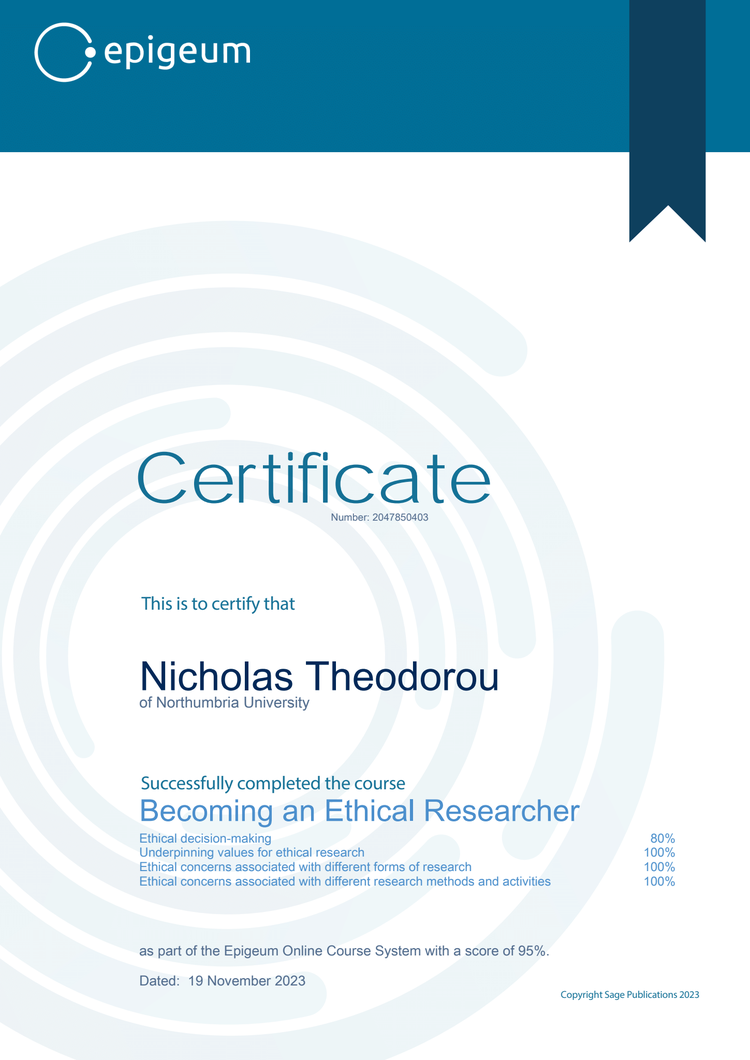
\includegraphics[width=14cm,height=8cm,keepaspectratio]{figures/introduction/ethics.png}
	\setlength\belowcaptionskip{3pt}
	\caption{Certificate of completion}
	\label{some-figure}
\end{figure}


% \section{Literary influences}

% First tranche of literature to review:

% Guo2023 \cite{Guo2023}
% Cie2022:\cite{Cie2022}
% Manohar2019: \cite{Manohar2019}
% Woolf2018: \cite{Woolf2018}
% Ghanekar2016: \cite{Ghanekar2016}
% Zhao2013: \cite{Zhao2013}
% Shemelya2014: \cite{Shemelya2014}
% Wu2012: \cite{Wu2012}
% Chen2012: \cite{Chen2012}
% Pendry2006: \cite{Pendry2006}
% Leonhardt2006: \cite{Leonhardt2006}
% Zhang2011: \cite{Zhang2011}
% Smith2005: \cite{Smith2005}
% Bernd2012: \cite{Bernd2012}
% Lan2013: \cite{Lan2013}
% Patel2021: \cite{Patel2021}
% Pendry1996: \cite{Pendry1996}
% Wang2016: \cite{Wang2016}
% Smith2002: \cite{Smith2002}
% Mandal2021: \cite{Mandal2021}
% Sreekanth2019: \cite{Sreekanth2019}
% Gholipour2018: \cite{Gholipour2018}
% Krishnamoorthy2018: \cite{Krishnamoorthy2018}
% Szymanski2023: \cite{Szymanski2023}
% Wang2008: \cite{Wang2008}
% Lu2021: \cite{Lu2021}
% Silva2019: \cite{Silva2019}
% Yousuf2021: \cite{Yousuf2021}
% Sun2022: \cite{Sun2022}
% Raju2020: \cite{Raju2020}
% Damour1996: \cite{Damour1996}
% Singh2019: \cite{Singh2019}
% Gregory2022: \cite{Gregory2022}
% Hasan2017: \cite{Hasan2017}
% LaPotin2022: \cite{LaPotin2022}
% Wen2010: \cite{Wen2010}
% Busch2007: \cite{Busch2007}
% Klein2006: \cite{Klein2006}
% Gentile2011: \cite{Gentile2011}
% Klein2006: \cite{Klein2006}
% Enkrich2005: \cite{Enkrich2005}
% Guo2020: \cite{Guo2020}
% Enkrich2005: \cite{Enkrich2005}
% Qin2022: \cite{Qin2022}
% Ferrari2015: \cite{Ferrari2015}
% Chen2023: \cite{Chen2023}
% Ma2023: \cite{Ma2023}
% Karami2021: \cite{Karami2021}
% Beliaev2021: \cite{Beliaev2021}
% Huo2019: \cite{Huo2019}
% Beliaev2021: \cite{Beliaev2021}
% Yan2022: \cite{Yan2022}
% Yang2018: \cite{Yang2018}
% Fan2022: \cite{Fan2022}
% Kuznetsov2023: \cite{Kuznetsov2023}
% Khatib2021: \cite{Khatib2021}
% Nadell2019: \cite{Nadell2019}
% Padilla2006: \cite{Padilla2006}
% Padilla2005: \cite{Padilla2005}
% Terekhov2019: \cite{Terekhov2019}
% Alabastri2013: \cite{Alabastri2013}
% Boltasseva2008: \cite{Boltasseva2008}
% Ghasemi2023: \cite{Ghasemi2023}
% Fang2023: \cite{Fang2023}
% Head2022: \cite{Head2022}
% Roberts2021: \cite{Roberts2021}
% Pareek2020: \cite{Pareek2020}
% Karami2021: \cite{Karami2021}
% Vafapour2021: \cite{Vafapour2021}
% Ghodsi2020: \cite{Ghodsi2020}
% Abdullahi2022: \cite{Abdullahi2022}
% Overview1998: \cite{Overview1998}
% Yin2015: \cite{Yin2015}
% Abdulkarim2022: \cite{Abdulkarim2022}
% Jahan2023: \cite{Jahan2023}
% Wu2021: \cite{Wu2021}








% % \lipsum[1]

% % \begin{itemize}
% % 	\item Item number one, 
% % 	\item item number two, 
% % 	\item item number three, 
% % \end{itemize}

% % \lipsum[3]
% % \vspace{7pt}
% % \begin{table}[!h]
% % 	\centering
% % 	\ra{1.1}
% % 	\caption{List of conferences at which I presented the results of investigations in the form of an oral presentation. }
% % 	\label{conferences} 
% % 	\vspace{-5pt}
% % 	\begin{tabular}{@{}lp{0.12\linewidth}p{0.25\linewidth}p{0.45\linewidth}@{}}
% % 		\doublerule
% % 		Date             & Place               & Conference                                                                                     & Title of contribution                                                                                                                         \\ \midrule
% % 		01.2026     & virtual   & A fancy Seminar                                                  & Really long name of the presentation \\
% % 		06.2027     & virtual   &  Conference  number two                                               & something equally interesting               \\
% % 		06.2029     & New York   & 11th International Conference                                                   & The same speech   \\
% % 		06.2029     & Copenhagen   & Nanotechnology conference          & A revolutionary presentation       \\
% % 		\bottomrule 
% % 	\end{tabular}
% % \end{table}












\end{document}
